% Created 2022-11-13 Sun 10:29
% Intended LaTeX compiler: xelatex
\documentclass[11pt]{article}
\usepackage{graphicx}
\usepackage{longtable}
\usepackage{wrapfig}
\usepackage{rotating}
\usepackage[normalem]{ulem}
\usepackage{amsmath}
\usepackage{amssymb}
\usepackage{capt-of}
\usepackage{hyperref}
\input{~/.config/latex/hebrew-latex.tex}
\author{Ido Merenstein}
\date{\today}
\title{Numerical Formula Sheet}
\hypersetup{
 pdfauthor={Ido Merenstein},
 pdftitle={Numerical Formula Sheet},
 pdfkeywords={},
 pdfsubject={},
 pdfcreator={Emacs 28.2 (Org mode 9.6)}, 
 pdflang={Hebrew}}
\begin{document}

\maketitle
\tableofcontents



\section{פירוק LU}
\label{sec:orge7cf14a}
\subsection{מטריצה משולשת תחתונה בסיסית}
\label{sec:orgeb94745}
\begin{itemize}
\item כל איברי אלכסונה 1
\item משולשת תחתונה
\end{itemize}

\subsection{מטריצה רגילה}
\label{sec:orge91918e}
ריבועית, \textbf{\textbf{וניתן}} לפרקה למכפלה מהצורה \(A=LU\)
(L משולשת תחתונה בסיסית, U משולשת עליונה כלשהי עם \textbf{\textbf{איברי אלכסון שונים מ-0}}).

\subsection{שימוש בפרמוטציה לפירוק \(LU\)}
\label{sec:orgd211b45}
נבצע את תהליך הדירוג כרגיל.

בכל פעם שניתקל באיבר ציר בעייתי, נחליף את השורה בה נמצא באחת השורות מתחתיו (ע״י כפל במטריצת פרמוטציה מתאימה).

כל מטריצה ריבועית \(A\) ניתנת לפירוק מהצורה \(PA=LU\), כאשר \(U\) לאו דוקא מדרגה מלאה.

\subsection{שימוש ב-LU לפתרון מערכת משוואות}
\label{sec:org8c61e76}
ע״י הקשר: \(\underline{b} = A \underline{x} = LU \underline{x} = L \left( U \underline{x} \right) = L \underline{y}\)

\begin{enumerate}
\item מציבים \(U\underline{x} = \underline{y}\) ופותרים \(L\underline{y} = \underline{b}\) ע״י החלפה קדמית.
\item פותרים \(U\underline{x} = \underline{y}\) ע״י החלפה אחורית.
\end{enumerate}

\subsection{מטריצות לא ריבועיות}
\label{sec:org64b7b0b}
\begin{center}
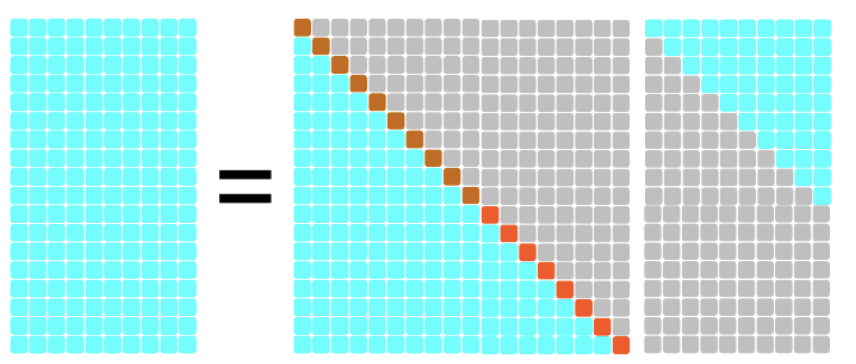
\includegraphics[width=.9\linewidth]{./img/m<n.png}
\end{center}
\begin{center}
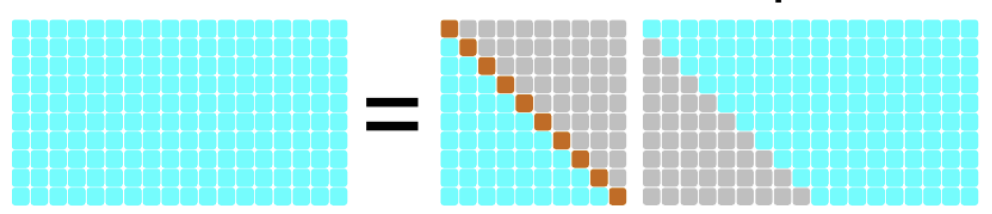
\includegraphics[width=.9\linewidth]{./img/m>n.png}
\end{center}

\subsection{שיטות לבחירת Pivot מוצלח}
\label{sec:org3e87a4b}
\begin{itemize}
\item \uline{Partial Pivoting} - בוחרים את איבר הציר להיות הגדול ביותר בעמודתו (ע״י פרמוטציה לשורות).
\item \uline{Full Pivoting} - בוחרים את איבר הציר להיות הגדול ביותר ביתרת המטריצה (ע״י פרמוטציה לשורות לעמודות).
\end{itemize}

\subsection{פירוק LDV}
\label{sec:org57a5b6c}
כל מטריצה \(A\) ריבועית שאינה סינגולרית ניתנת לפירוק מהצורה \(PA=LDV\) כאשר:
\begin{itemize}
\item \(P\) מטריצת פרמוטציה שמחליפה סדר שורות
\item \(L\) מטריצה משולשת תחתונה בסיסית
\item \(D\) מטריצה אלכסונית בה כל האיברים שונים מ-0
\item \(V\) מטריצה משולשת עליונה בסיסית
\end{itemize}

\subsection{פירוק \(LDL^{T}\) קיים למטריצות חיוביות מוגדרות}
\label{sec:org1aba0a5}
מטריצה סימטרית וחיובית מוגדרת \(A\) היא בהכרח מטריצה רגילה,
וקיים עבורה פירוק \(A=LDL^T\) ללא צורך בפרמוטציה, עם אלכסון מטריצה \(D\) חיובי ממש.
בפרט ניתן לרשום שקיימת \(M\) משולשת תחתונה עם אלכסון חיובי, כך ש-\(A = MM^T\).


\subsection{אלגוריתם יעיל לפירוק \(LU\)}
\label{sec:orgb37cd03}


\section{ריבועים פחותים}
\label{sec:orgc7da0de}

\subsection{סימון בעיית ריבועים פחותים כבעיה ריבועית}
\label{sec:org23d1d11}
מתקיים:
\[
\|A\underline{x} - \underline{b}\|_2^2
=
\underline{x}^TK\underline{x} - 2\underline{x}^T\underline{f}+c
\]

כאשר:
\begin{itemize}
\item \(K = A^TA\)
\item \(\underline{f} = A^T\underline{b}\)
\item \(c=\underline{b}^T\underline{b}\)
\end{itemize}

\subsection{מציאת מינימום של בעיה ריבועית}
\label{sec:org01cb1ce}

בהינתן הבעיה הריבועית \(p \left( \underline{x} \right) = \underline{x}^TK\underline{x} - 2\underline{x}^T\underline{f} + c\),

אם \(K\) חיובית מוגדרת, אז ל-\(p \left( \underline{x} \right)\) נקודת מינימום \uline{יחידה וגלובלית} שנתונה ע״י: \(\underline{x}^{*}=K^{-1}\underline{f} = A^{\dagger} \underline{b}\)

וערך הפונקציה במינימום הוא: \(p \left( \underline{x} \right) = c - \left( \underline{x}^* \right)^TK \left( \underline{x}^{*} \right)\)

אם \(K\) חיובית חצי-מוגדרת, אז כל וקטור שמקיים את המשוואה:
\(K\underline{x}^{*} = \underline{f}\)

יהווה פתרון אופטימלי לבעיה, עם ערך מינימום של \(p \left( \underline{x} \right) = c - \left( \underline{x} \right)^TK \left( \underline{x}^{*} \right)\).

\subsection{התאמת עקומות לנתונים}
\label{sec:orgfc00ddb}
\subsection{ריבועים פחותים ממושקלים}
\label{sec:orgeb8e6d1}
בעיה שבה צריך להביא למינימום ביטוי מהצורה:

$$\left( A\underline{x} - b \right)^T W \left( A\underline{x} - \underline{b} \right)
=
\|A\underline{x}-\underline{b}\|_W^2$$

כאשר איברי האלכסון של המטריצה האלכסונית \(W\) חיוביים ממש.

הפתרון \(x^{*}\) חייב לקיים: \(A^TWA\underline{x}^{*} = A^TW\underline{b}\)

\subsection{רגולריזציה לבעיות LS}
\label{sec:orgdf75198}
לבעיה הריבועית הבאה עם  \(\lambda>0\):
\[
\min_{\underline{x}} \|A\underline{x}-\underline{b}\|_2^2 + \lambda \|\underline{x}\|^2_2
\]

יש פתרון יחיד שנתון על ידי:
\[
\underline{x}^{*} = \left( A^TA + \lambda I \right)^{-1} A^T\underline{b}
\]

\uline{גרסה כללית יותר:}

\[
\left( A^TA + \lambda C^TC \right)\underline{x}^{*} = A^T\underline{b}
\impliedby
\min_{\underline{x}} \|A\underline{x}-\underline{b}\|_2^2 + \lambda \|C\underline{x}\|_2^2
\]
אם \(C^TC\) חיובית מוגדרת, הפתרון לבעיה יהיה יחיד.



\section{אורתוגונליות ופירוק \(QR\)}
\label{sec:org3e65c94}
\subsection{תכונות של מטריצות אורתונורמליות}
\label{sec:org2f4bf82}
לכל מטריצה אורתונורמלית \(Q\):
\begin{itemize}
\item \(Q^{-1} = Q^T\)
\item \(\det \left( Q \right) = \pm 1\)
\item \(\|Q \underline{x}\|_2^2 = \|\underline{x}\|_2^2\)
\item מכפלת מטריצות אורתונורמליות היא אורתונורמלית
\end{itemize}

\subsection{תהליך Gram-Schmidt}
\label{sec:orgc3f9ae5}
בהינתן סט וקטורים בת״ל \(\left\{ \underline{w}_k \right\}_{k=1}^L \in \mathbb{R}^n\), קיים בסיס אורתונורמלי \(\left\{ \underline{u}_k \right\}_{k=1}^L \in \mathbb{R}^n\) כך שמתקיים:
\[
\text{span} \left\{ \underline{w}_1, \underline{w}_2, \ldots, \underline{w}_n \right\}
=
\text{span} \left\{ \underline{u}_1, \underline{u}_2, \ldots, \underline{u}_{L} \right\}
\]

\subsubsection{אלגוריתם Gram-Schmidt}
\label{sec:org179f474}
\uline{אתחול:}
\begin{itemize}
\item קבע \(k=1\)

\item הבא את הווקטור \(\underline{w}_1\)
\end{itemize}

\uline{איטרציה:}
\begin{itemize}
\item קילוף: \(\underline{u}_k = \underline{w}_k - \sum_{j=1}^{k-1} \left( \underline{u}_j^T\underline{w}_k \right) \underline{u}_j\)

\item נרמול: \(\underline{u}_k = \frac{\underline{u}_k}{\|\underline{u}_k\|_2}\)

\item קבע \(k=k+1\)

\item הבא את הווקטור \(\underline{w}_k\)
\end{itemize}

\subsubsection{אלגוריתם Modified Gram-Schmidt}
\label{sec:orgb95db2c}
\subsubsection{אלגוריתם Stable Gram-Schmidt}
\label{sec:org5a4cc0d}

\subsection{פירוק QR}
\label{sec:orgf29697f}
\subsubsection{למטריצות ריבועיות}
\label{sec:org281cf63}
\begin{enumerate}
\item למטריצות הפיכות
\label{sec:org04791bb}
כל מטריצה ריבועית ולא סינגולרית \(A\) ניתנת לפירוק \textbf{יחיד} מהצורה \(A=QR\), כאשר
\begin{itemize}
\item \(Q\) מטריצה אורתונורמלית
\item \(R\) משולשת עליונה עם איברי אלכסון ראשי חיוביים
\end{itemize}

\item למטריצות סינגולריות
\label{sec:org431f867}
עוברים על העמודות ומבצעים תהליך GS. אם מוצאים עמודה שתלויה בקודמיה:
\begin{itemize}
\item מייצגים אותה כצירוף של הווקטורים שכבר נוצרו (כעמודה ב-\(R\))
\item מגרילים וקטור חדש שימלא את מקומה להמשך תהליך GR (ינורמל וימוקם ב-\(Q\)).
\end{itemize}
\end{enumerate}

\subsubsection{למטריצות מלבניות}
\label{sec:org56354b2}
\begin{itemize}
\item עבור מטריצה רחבה ונמוכה, העמודות חייבות להיות ת״ל.
אם נניח ש-\(n\) העמודות הראשונות בת״ל, נקבל שעמודות \(R\) מלאות.
\end{itemize}

\begin{center}
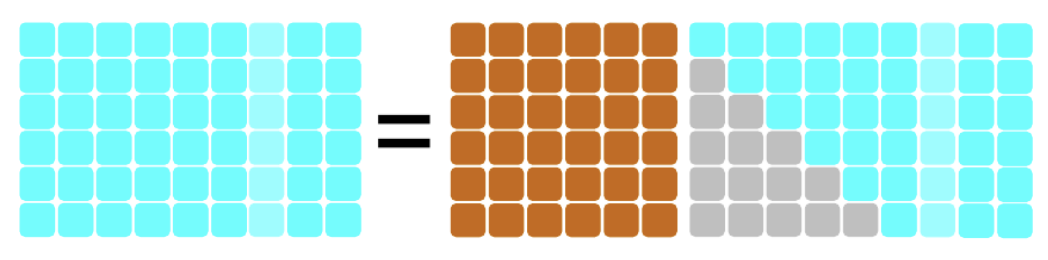
\includegraphics[width=.9\linewidth]{./img/QR-wide-short.png}
\end{center}

\begin{itemize}
\item עבור מטריצה גבוהה וצרה, ניתן להציע שני מבני פירוק:
\begin{itemize}
\item \(Q\) מלאה עם וקטורי סרק שהוספו לצורך יצירת מטריצה אורתונורמלית.
\item מטריצה שבה מסתפקים ב-\(Q\) ברוחב של \(A\) (Economy QR).
\end{itemize}
\end{itemize}

\begin{center}
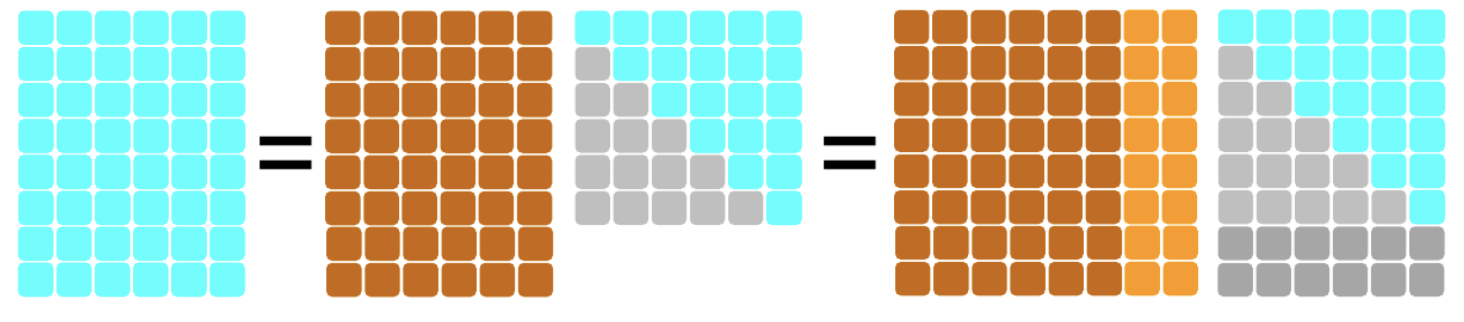
\includegraphics[width=.9\linewidth]{./img/QR-tall-narrow.png}
\end{center}

\subsection{שימור ב-QR לפתרון LS}
\label{sec:org7fbfc3a}


\section{ערכים עצמיים וסינגולריים}
\label{sec:org89c97ee}

\subsection{הצמדת מטריצה משמרת ערכים עצמיים}
\label{sec:org3ed0aa4}
בהינתן מטריצה ריבועית \(A\) ומטריצה הפיכה \(G\) באותו גודל,
  המטריצה \(G^{-1}AG\) תהיה בעלת אותם ע״ע כשל \(G\) (הו״ע לאו דוקא זהים).

\subsection{פירוק Schur}
\label{sec:orgc46a927}
בהינתן מטריצה ריבועית \(A\) לכסינה, ניתן למצוא:
\begin{itemize}
\item מטריצה אורתונורמלית \(Q\)
\item מטריצה משולשת עליונה \(T\)

כך שמתקיים:
$$Q^TAQ=T$$

איברי האלכסון הראשי של \(T\) יהיו הערכים העצמיים של \(A\).
\end{itemize}

\subsection{לכסון מטריצה סימטרית ממשית (פירוק ספקטרלי)}
\label{sec:org726ff1d}
אם מטריצה \(A\) ריבועית ממשית וסימטרית, אזי:
\begin{itemize}
\item המטריצה בהכרח לכסינה
\item \textbf{כל ערכיה העצמיים ממשיים}
\item וקטוריה העצמיים מהווים סט אורתונורמלי, לכן ניתנת ללכסון אורתונורמלי: \(Q^TAQ=D\)
\end{itemize}

\subsection{חיוביות/אי-שליליות של ע״ע במטריצות סימטריות}
\label{sec:orgc0052ad}
\begin{itemize}
\item אם \(K\) סימטרית וחיובית מוגדרת, אז כל ערכיה העצמיים \textbf{חיוביים}.
\item אם \(K\) סימטרית חצי-מוגדרת, אז כל ערכיה העצמיים \textbf{אי-שליליים}.
\end{itemize}

\subsection{ע״ע כפתרון לבעיות אופטימיציה}
\label{sec:orga9b14c6}
למטריצה חיובית חצי מוגדרת \(A\) בגודל \(n\times n\) בעלת ערכים עצמיים \(\lambda_1 \ge \lambda_2 \ge \lambda_3 \ge \ldots \ge \lambda_n \ge 0\)
ווקטורים עצמיים תואמים \(\underline{v}_1, \underline{v}_2, \underline{v}_3, \ldots, \underline{v}_n\), מתקבל כי:

\begin{align*}
  \max_{\underline{x},\ \|\underline{x}\|_2=1} \underline{x}^TA\underline{x} = \lambda_1
&&
\arg \max_{\underline{x},\|\underline{x}\|_2=1} \underline{x}^TA\underline{x}=\underline{v}_n \\ \\
\min_{\underline{x},\ \|\underline{x}\|_2=1} \underline{x}^TA\underline{x} = \lambda_1
&&
\arg \min_{\underline{x},\|\underline{x}\|_2=1} \underline{x}^TA\underline{x}=\underline{v}_n
\end{align*}

\subsubsection{מנת ריילי}
\label{sec:org7555a17}



\[
\underline{x}^{*} = \arg \max_{\underline{x} \ne 0} \left( \frac{\underline{x}^TA\underline{x}}{\underline{x}^T\underline{x}} \right)
\]

\subsubsection{ערכים עצמיים מוכללים / עפרון}
\label{sec:org06ec5c2}
\[
\underline{x}^{*} = \arg \max_{\underline{x} \ne 0} \left( \frac{\underline{x}^TA\underline{x}}{x^TB\underline{x}} \right)
\]

\[
A\underline{x}= \lambda B\underline{x}
\impliedby
A\underline{x} = \left( \frac{\underline{x}^TA\underline{x}}{\underline{x}^TB\underline{x}} \right) B \underline{x}
\impliedby
\nabla \left( \frac{\underline{x}^TA\underline{x}}{\underline{x}^TB\underline{x}} \right) = 0
\]

כאשר \(B\) מטריצה חיובית מוגדרת.

\subsection{פירוק SVD}
\label{sec:org4edc126}

כל מטריצה ממשית \(A_{m \times n}\) ניתנת לפירוק \(SVD\) מהצורה:
\[
A = U\Sigma V^T = \sum_{k=1}^{r}\sigma_k \underline{u}_K \underline{v}_k^{T}
\]

כאשר:
\begin{itemize}
\item \(U\) מטריצה אורתונורמלית בגודל \(m \times m\).
\item \(\Sigma\) מטריצה אלכסונית בגודל \(m \times n\) (גודל \(A\)), כאשר איברי אלכסונה אי-שליליים ובמגמת ירידה, ונקראים \textbf{ערכים סינגולריים}.
\item \(V\) מטריצה אורתונורמלית בגודל \(n \times n\).
\end{itemize}

\subsection{שלבי הבנייה של פירוק SVD}
\label{sec:org426b392}
שלבי הבנייה עבור מטריצה \(A_{m \times n}\) מלבנית גבוהה (\(m>n\)) מדרגה מלאה:

\begin{enumerate}
\item חשב את המטריצה \(A^TA\).
\item בצע למטריצה זו פירוק ספקטרלי וקבל את \(\left\{ \lambda_k, \underline{v}_l \right\}_{k=1}^n\), \(v_i\) וקטורים א״נ.
\item אסוף את הווקטורים \(\underline{v}_i\) כשורותיה של מטריצה - זוהי \(V^T\).
\item הוצא שורש לע״ע \(\lambda_i\) ואלו יהיה \(\sigma_i = \sqrt{\lambda_i}\), איברי האלכסון של \(\Sigma\).
\item חשב \(\underline{u}_i = \frac{A\underline{v}_i}{\sigma_i}\) לכל \(1 \le i \le n\), אלו יהיו עמודות \(U\).
\item בנה את הווקטורים \(\underline{u}_k\) הנותרים ע״י תהליך GS ובנה מהם את החלק הנותר ב-\(U\) (כדי להשלימה לריבועית).
\end{enumerate}

עבור מטריצה מדרגה לא מלאה, ניתקע בשלב 5, ולכן נגריל את הווקטורים \(\underline{u}_{r+1}, \ldots, \underline{u}_n\) שעבורם \(\sigma_i = 0\),
ונבנה אותם באופן שרירותי כהמשך לבסיס הא״נ במטריצה \(U\).

עבור מטריצה מלבנית ״רחבה״ (\(m < n\)), נבצע את הפירוק \(A^T = U\Sigma V^T\) ונבצע שחלוף על אגפי המשוואה.

\subsection{פירוק SVD למטריצות סימטריות}
\label{sec:org2d9f120}
עבור מטריצות סימטריות PSD, פירוק ה-SVD שקול לפירוק הספקטרלי.

עבור מטריצה סימטרית שאינה PSD עם ע״ע \(\left\{  \lambda_i \right\}_{i=1}^n\), הערכים הסינגולריים יהיו \(\left\{  \sigma_i\right\}_{i=1}^n = \left\{  \left| \lambda_i \right|  \right\}_{i=1}^n\),

ועבור פירוק ספקטרלי \(A = QDQ^T\) נקבל:
\[
A = U\Sigma V^T = Q \left( D P \right) \left( P Q^{T} \right)
\]

כאשר \(P\) מטריצה אלכסונית שאחראית על היפוך הסימן בשורות שמתייחסות לע״ע שליליים ב-\(D\).

\begin{center}
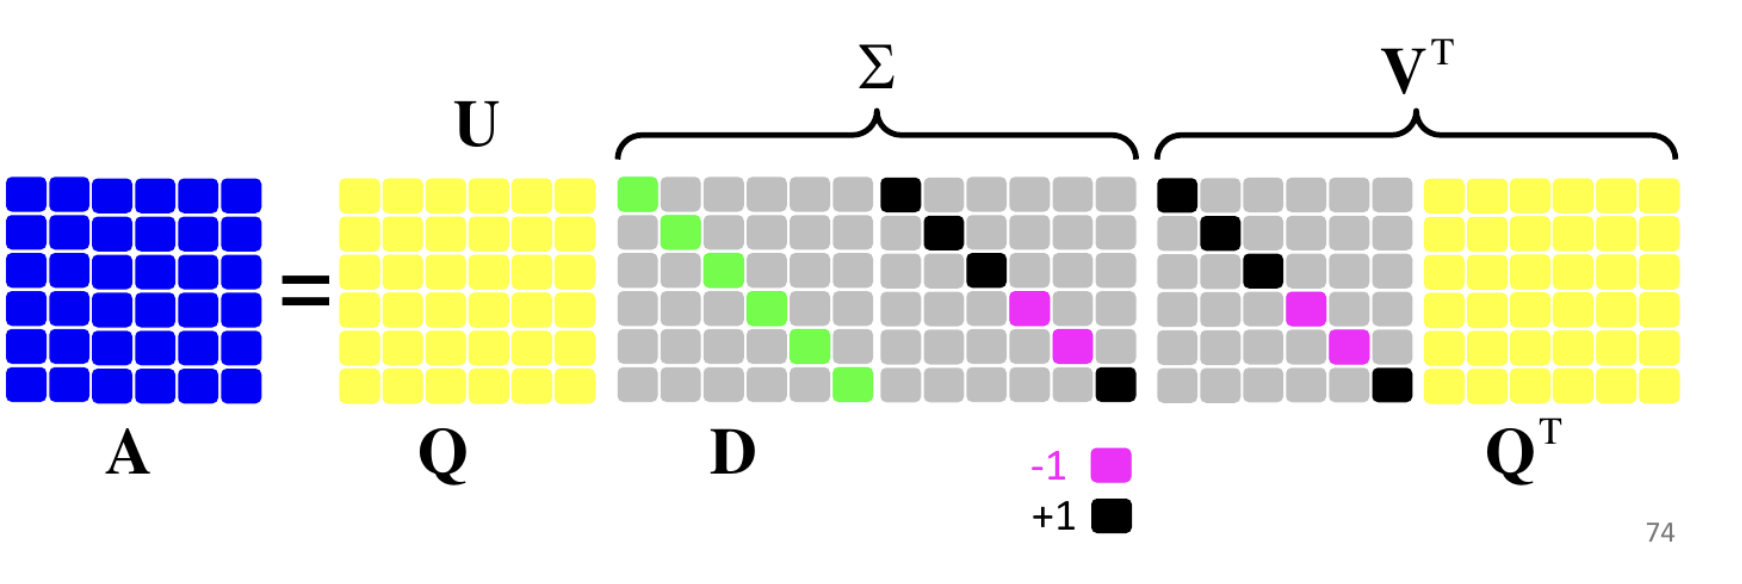
\includegraphics[width=.9\linewidth]{./img/specral-decomposition-non-psd.png}
\end{center}

\subsection{פתרון מערכות משוואות ע״י SVD}
\label{sec:org6d283d9}
נרצה לפתור את המערכת \(A\underline{x}= \left( U \Sigma V^T \right)\underline{x} = \underline{b}\).

\begin{itemize}
\item עבור \(A\) ריבועית והפיכה,
\[
  \underline{x} = \left( U \Sigma V^T \right)^{-1}\underline{b}
  =
  V \Sigma^{-1} U^T
  \]

\item עבור \(A_{m \times n}\) מלבנית גבוהה (\(m>n\)) מדרגה מלאה,
\[
  \underline{x} = V \Sigma^{-1} U^T
  \]

כאשר \(\Sigma^{-1}\) זו הכללה להיפוך של המטריצה \(\Sigma\), באופן הבא:
\end{itemize}

\begin{center}
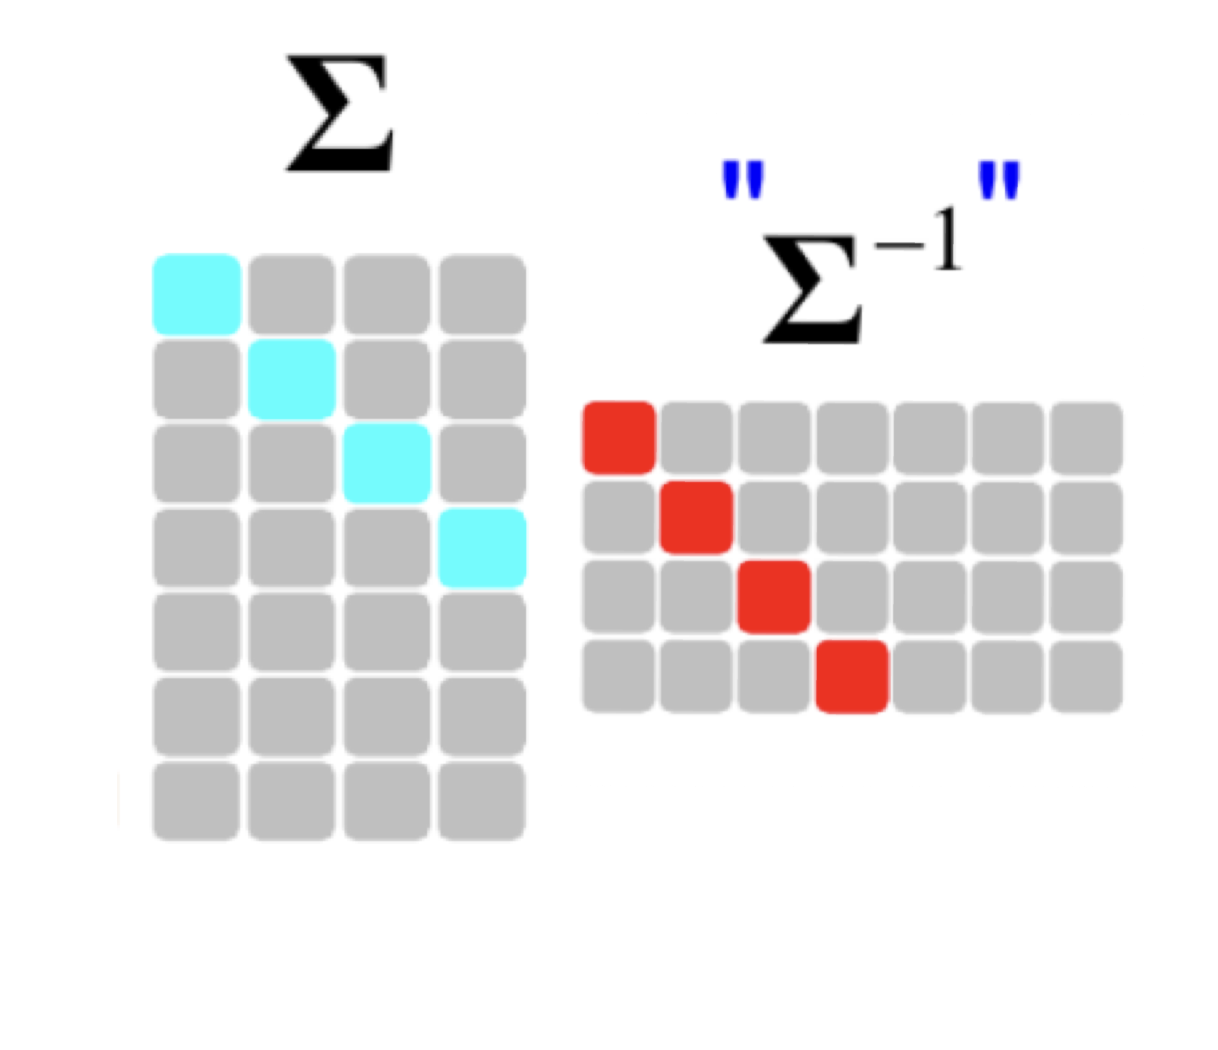
\includegraphics[width=.9\linewidth]{./img/generalized-sigma.png}
\end{center}

\begin{itemize}
\item עבור \(A_{m \times n}\) מלבנית רחבה (\(m < n\)) מדרגה מלאה,
\begin{itemize}
\item מגדירים \(\underline{z}=V^T\underline{x}\)
\item פותרים \(\Sigma \underline{z}=U^T\underline{b}\)
\item הפתרון הוא \(\underline{x}=V\underline{z}\)

\item נגלה עניין מיוחד בפתרון שתחתיתו אפסים
\item הפתרון הקצר ביותר עבור \(\underline{z}\) מוביל לפתרון הקצר ביותר עבור \(\underline{x}\) (\(V\) מטריצה א״נ).

ניתן גם לכתוב ע״י  \(\underline{x}=V\ "\ \Sigma^{-1}\ "\ U^T\) ע״י הכללת היפוך של \(\Sigma\):
\end{itemize}
\end{itemize}
\begin{center}
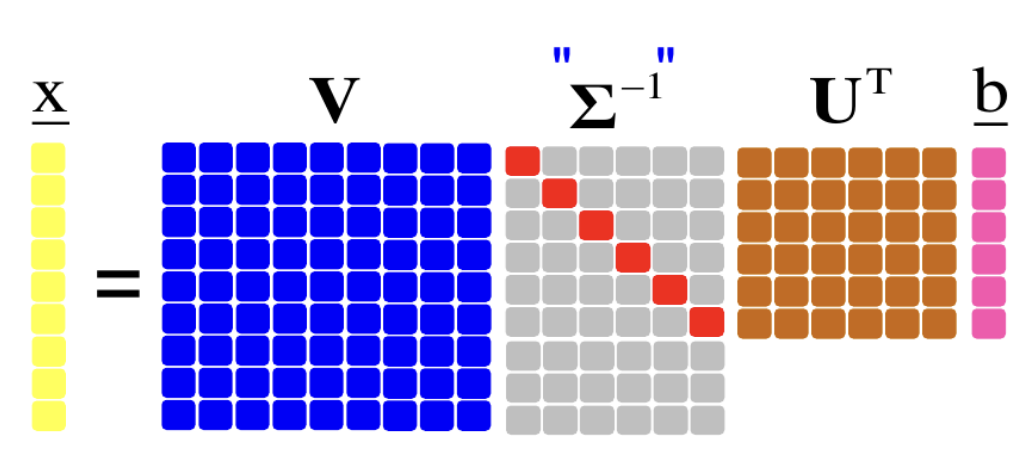
\includegraphics[width=.9\linewidth]{./img/wide-matrix-svd-sys.png}
\end{center}

\subsection{פתרון ריבועים פחותים ע״י SVD}
\label{sec:orgbaa7cdf}
עבור הבעיה \(\min_{\underline{x}}\|A\underline{x}-\underline{b}\|_2^2\) עם מטריצה \(A_{m \times n}\),

\begin{itemize}
\item הפתרון האופטימלי עבור בעיית LS עם פתרון יחיד יהיה: \(\underline{x}_{\text{opt}} = A^{\dagger}\underline{b} = V\Sigma^{\dagger}U^T\underline{b}\).

\item עבור בעיה עם אינסוף פתרונות (\(\text{rank} \left( A \right) < n\)), המשוואה הנורמלית תהיה:
\[
    \Sigma^T\Sigma V^T\underline{x}
    =
    \fbox{$\Sigma^T\Sigma \underline{z}
    =
    \Sigma^T \hat{b}$}
    =
    \Sigma^TU^T\underline{b}
  \]

נקבל וקטור פתרון \(\underline{z}\) שעבורו כל רכיב \(1 \le i \le r\) הוא \(z_i = \frac{\hat{b}_i}{\sigma_i}\), כאשר \(\sigma_r\) הע״ס המינימלי ששונה מאפס, ולכל \(r < i \le n\) יש חופש בבחירת \(z_{i}\).

אם משתמשים בהגדרת היפוך מוכלל של מטריצה אלכסונית, הפתרון \(\underline{x}_{opt}=V\Sigma^{\dagger}U^T\underline{b}\) הופך לוואלידי, במשמעות של ״הפתרון הקצר ביותר״
\end{itemize}

\subsection{פתרון מאוחד לשני סוגי הבעיות}
\label{sec:org7a09e78}
\(\underline{x}_{opt}=V\Sigma^{\dagger}U^T\underline{b}\) הוא פתרון שמתאים גם עבור הבעיה \(A\underline{x}=\underline{b}\) וגם עבור \(min_{\underline{x}}\|A\underline{x}-\underline{b}\|_2^2\).

\begin{itemize}
\item במקרה של פתרון יחיד, זהו הפתרון המדויק.
\item במקרה של \(\infty\) פתרונות, זהו הפתרון הקצר ביותר.
\end{itemize}

\subsection{קירוב מטריצות עם אילוץ דרגה}
\label{sec:orgf7a60ec}
עבור מטריצה \(A = U \Sigma V^T = \sum_{k=1}^{r}\sigma_k \underline{u}_k \underline{v}_k^T\) עם ע״ס \(\sigma_1 \ge \sigma_2 \ge \ldots \ge \sigma_r > 0\),

פתרון הבעיה  \(\min_B \|A - B\|_F^2\ \  s.t.\ \  \text{rank} \left( B \right) = k_0\) הינו \(B=\sum_{k=1}^{k_0}\sigma_k \underline{u}_k \underline{v}_k^T\).

כאשר \(\|A - B\|_F^2 = \sum_{k = k_0+1}^{r}\sigma_k^2\).


\section{תהליכים איטרטיביים}
\label{sec:org448b212}
\subsection{מערכת דינמית}
\label{sec:org614f88f}
מערכת שיוצרים סדרה אינסופית של וקטורים \(u_k\) באופן הבא:

\[
\underline{u}_k = \begin{cases}
T \cdot \underline{u}_{k-1} & k \ne 0 \\
\underline{u}_0 & k = 0
\end{cases}
\ \ =\ \
T^k \cdot\underline{u}_{0}
\]

כאשר \(T\) מטריצה קבועה כלשהי ו-\(\underline{u}_0\) וקטור התחלתי.

\subsection{מערכת דינמית של מטריצה לכסינה}
\label{sec:org16ac5fc}
איבר \(\underline{u}_k\) נתון ע״י הנוסחה:

\[
\underline{u}_k = T^k\underline{u}_0
=
V \Lambda^kV^{-1}\underline{u}_0
=
V \Lambda^k\underline{x}_0
=
\sum_{j=1}^{n}x_0 \left( j \right) \cdot \lambda_j^k \cdot \underline{v}_j
\]

כאשר \(\underline{x}_0 \triangleq V^{-1}\underline{u}_0\).
\subsection{מערכת דינמית יציבה אסימפטוטית}
\label{sec:orgd79d0cc}
מערכת דינמית מהצורה \(\underline{u}_k = T \underline{u}_{k-1} = T^k \underline{u}_0\) תיקרא \textbf{יציבה אסימפטוטית}

אם מתקיים כי  \(\underline{u}_k \underset{k \to \infty}{\longrightarrow}\underline{0}\).

\subsection{מטריצה יציבה}
\label{sec:orge574abe}
מטריצה \(T\) תיקרא \textbf{יציבה} אם \(T^k \underset{k \to \infty}{\longrightarrow} 0\).

\subsection{רדיוס ספקטרלי}
\label{sec:org491fa35}
בהינתן מטריצה \(T\) כלשהי, \textbf{הרדיוס הספקטרלי} שלה מוגדר להיות:
\[
\rho \left( T \right) = \max_{1 \le k \le n} \left| \lambda_k \right| = \lambda_1
\]

\uline{תיאור גרפי:} הרדיוס של הדיסקה שמרכזה בראשית הצירים שמכסה את כל הע״ע של \(T\).
\begin{center}
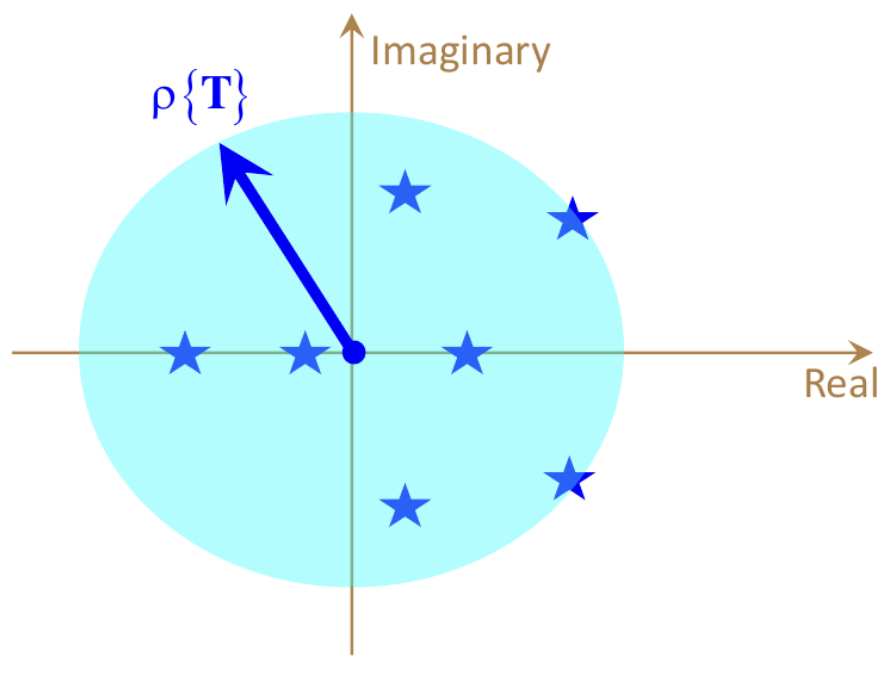
\includegraphics[width=.9\linewidth]{./img/specral-radius-disc.png}
\end{center}

\subsection{מערכת של מטריצה לכסינה \(T\) עם \(\rho \left( T \right) < 1\) יציבה אסימפטוטית}
\label{sec:orgc008bb2}

אם \(T\) לכסינה ובנוסף \(\rho \left( T \right) < 1\), אז המערכת הדינמית \(\underline{u}_k = T^k\underline{u}_0\) יציבה אסימפטוטית, כאשר:
\[
\forall j \in \left[ 1, n \right]\ \ \left| \lambda_j \right| < 1
\iff
\rho \left( T \right) < 1
\]

\subsection{קצב התכנסות}
\label{sec:org11171b3}
לכל \(k \in \mathbb{N}\) מתקיים \(\|u_k\|_2 \le C \cdot \rho \left( T \right)^k\) עבור \(C>0\) מסוים, ולכן:
\begin{itemize}
\item ככל שהרדיוס הספקטרלי קטן יותר, ההתכנסות אל האפס תהיה מהירה יותר.
\item ככל שהרדיוס הספקטרלי קרוב ל-1, ההתכנסות אל האפס תהיה איטית יותר.
\end{itemize}


\subsection{הגדרה של נורמה}
\label{sec:orge5a38a6}
עבור מרחב וקטורי \(V\) מעל שדה \(\mathbb{F}\), \textbf{נורמה} היא פונקציה \(\|\mathord{\cdot}\| : V \to \mathbb{R}^{+}\) המקיימת:
\begin{enumerate}
\item (\emph{חיוביות לחלוטין}) \(\forall v \in V : \|\underline{v}\| \ge 0,\ \ \ \|\underline{v}\| = 0 \iff \underline{v} = 0\)
\end{enumerate}


\begin{enumerate}
\item (\emph{הומוגניות}) \(\forall \underline{v} \in V,\ \ \forall \alpha \in \mathbb{F}:\ \|\alpha \underline{v}\| = \left| \alpha \right| \cdot \|\underline{v}\|\)
\end{enumerate}


\begin{enumerate}
\item (\emph{אי-שוויון המשולש}) \(\forall \underline{u},\underline{v} \in V:\ \ \|\underline{u} + \underline{v}\| \le \|\underline{u}\| + \|\underline{v}\|\)
\end{enumerate}

\subsection{נורמות ידועות}
\label{sec:org522fd17}
\begin{itemize}
\item נורמת פורביניוס:
\end{itemize}
\[
\|E\|_F = \sqrt{\sum_{k=1}^m \sum_{j=1}^{n}e_{kj}^2} = \sqrt{\text{trace} \left( E^TE \right)}
=
\sqrt{\text{trace} \left( \Sigma^T\Sigma \right)}
=
\sqrt{\sum_{k=1}^n \sigma_k^2}
\]

\begin{itemize}
\item נורמת \(L^2\):
\end{itemize}
\[
\|\underline{x}\|_2 = \sqrt{\underline{x}^T\underline{x}} = \sqrt{\sum_{k=1}^n \left| x_k \right|^2}
\]

\begin{itemize}
\item נורמת \(WL^2\) (\(L^{2}\) ממושקלת):
\end{itemize}
\[
\|\underline{x}\|_W = \sqrt{\underline{x}^TW\underline{x}} = \sqrt{\sum_{k=1}^n w_k \left| x_k \right|^2}, \ \ w_k > 0\ \ \  \forall 1 \le k \le n
\]
\begin{itemize}
\item נורמת \(L^1\):
\end{itemize}
\[
  \|\underline{x}\|_1 = \sum_{k=1}^{n} \left| x_k \right|
\]

\begin{itemize}
\item נורמת \(L^{\infty}\):
\end{itemize}
\[
\|\underline{x}\|_{\infty} = \max_{1 \le k \le n} \left| x_k \right|
\]

\begin{itemize}
\item נורמת \(L^{p}\) עבור \(p \ge 1\):
\end{itemize}
\[
\|\underline{x}\|_p = \left( \sum_{k=1}^{n} \left| x_k \right|^p \right)^{\frac{1}{p}}
\]

\subsection{משפט שקילות הנורמות}
\label{sec:orgd96a718}
בהינתן שתי נורמות \(\|\mathord{\cdot}\|_{A}\), \(\|\mathord{\cdot}\|_B\) המוגדרות על וקטורים באורך \(n\),

קיימים בהכרח שני קבועים \(0 < c_1 < c_2 < \infty\) כך שמתקיים:
\[
\forall \underline{v},\ \ c_1 \|\underline{v}\|_A \le \|\underline{v}\|_B \le c_2 \|\underline{v}\|_A
\]

\subsubsection{מסקנה: התכנסות גודל סדרת וקטורים לאפס לא תלויה בנורמה}
\label{sec:orgf0dc5ed}
בהינתן שתי נורמות \(\|\mathord{\cdot}\|_{A}\), \(\|\mathord{\cdot}\|_B\) המוגדרות על וקטורים באורך \(n\), וסדרת וקטורים \(\left\{ v_k \right\}_{k=0}^{\infty}\), מתקיים:

\[
\|\underline{v}_k\|_A \underset{k \to \infty}{\longrightarrow} \underline{0}
\ \ \ \iff\ \ \
\|\underline{v}_k\|_B \underset{k \to \infty}{\longrightarrow} \underline{0}
\]

\subsection{נורמה של מטריצה ריבועית}
\label{sec:org7951e97}
בהינתן נורמה \(|\mathord{\cdot}\|_{A}\) המוגדרת על וקטורים באורך \(n\), נורמה של המטריצה \(T_{n \times n}\) מוגדרת להיות:
\[
\left| \|T\| \right|_A
\triangleq
\max_{\underline{v}, \|\underline{v}\|_A = 1} \|T \underline{v}\|_A
=
\max_{\underline{v} \ne 0} \frac{\|T \underline{v}\|_A}{\| \underline{v}\|_A}
\]

\subsubsection{תכונות של נורמה של מטריצה}
\label{sec:orge10d033}

\begin{enumerate}
\item (\emph{פירוק מכפלה מטריצית-וקטורית}) - \(\|T \underline{v}\|_A = \left|\|  T \|\right|_A \|\underline{v}\|_{A}\)

\item (\emph{פירוק מכפלה מטריצית-מטריצית}) - \(\left| \|T_1T_2\| \right|_A = \left| \|T_1\| \right|_A \left| \|T_2\| \right|_{A}\)

\item (\emph{קיום נורמה מטריצית קטנה מ-\(1\) מבטיחה התכנסות אסימפטוטית של מערכת דינמית})

עבור מערכת דינמית \(\underline{u}_k = T^k\underline{u}_0\) ונורמה \(\|\mathord{\cdot}|_{A}\), אם מתקיים כי \(\left| \|T\| \right|_A < 1\), אזי המערכת מובטחת להתכנס אסימפטוטית,

כאשר \(T\) היא לאו דוקא לכסינה.

\item (\emph{הרדיוס הספקטרלי הוא חסם תחתון לכל הנורמות המטריציות})

לכל נורמה \(\|\mathord{\cdot}|_{A}\) ומטריצה \(T\) ריבועית מתקיים: \(\rho \left( T \right) \le \| \left| T \right|\|_A\).

\begin{itemize}
\item מסקנה: אם קיימת \(\| \left| T \right|\|_A < 1\), אז מובטח ש-\(\rho \left( T \right) < 1\).
\end{itemize}
\end{enumerate}

\subsubsection{נוסחאות לנורמות מטריציות מוכרות}
\label{sec:org3f97417}

\begin{itemize}
\item \uline{נורמת אינסוף מטריצית}:
\end{itemize}

\[
\left| \|T\| \right|_{\infty} = \max_k \left\{ \sum_{j=1}^{n} \left| t_{kj} \right| \right\}
\]

סכום שורה מקסימלי.

\begin{itemize}
\item \uline{נורמת 1 מטריצית}:
\end{itemize}

\[
\left| \|T\| \right|_1
=
\max_{\ell} \left\{ \sum_{k=1}^{n} \left| t_{k\ell} \right| \right\}
\]

סכום עמודה מקסימלי.

\begin{itemize}
\item \uline{נורמת 2 מטריצית}:
\end{itemize}

\[
\left| \|T\| \right|_2 = \sigma_1
\]

הערך הסינגולרי הגדול ביותר של \(T\).

\textbf{נשים לב שנורמת פורביניוס חוסמת מלמעלה את נורמת 2 מטריצית}:
\[
\|T\|_F =  \sqrt{\sum_{k=1}^n \sigma_k^2} \ge \sigma_1 =  \left| \|T\| \right|_2
\]

\subsection{משפט גרשגורן}
\label{sec:org42a68fd}

עבור \(T_{n \times n}\) מטריצה ריבועית, נגדיר \(n\) דיסקאות \(D_k,\ \ 1 \le k \le n\) באופן הבא:
\[
D_k
=
\left\{ z \in \mathbb{C} \mid \left| z - t_{kk} \right|
\le \sum_{j \ne k} \left| t_{kj} \right| \right\}
\]

(כל דיסקה נוצרת משורה אחת ב-\(T\), שמרכזה הוא \emph{איבר האלכסון}, ורדיוסה הוא \emph{סכום יתר האיברים בערך מוחלט}.)

אזי כל הערכים העצמיים של \(T\) מוכלים באיחוד של דיסקאות אלו.

\begin{center}
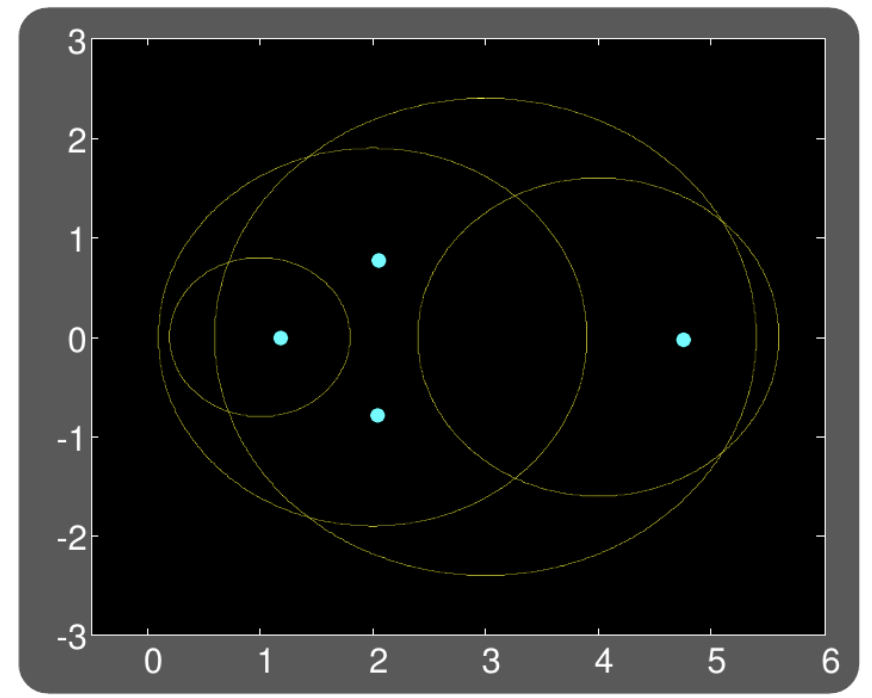
\includegraphics[width=.9\linewidth]{./img/gershgoren-representation.png}
\end{center}

\subsection{מטריצה דומיננטית באלכסון}
\label{sec:org547597a}
מטריצה \(T\) נקראת \textbf{דומיננטית באלכסון} אם כל איבר אלכסון בה גדול ממש (בערך מוחלט) מסכום יתר האיברים בשורתו:
\[
\forall 1 \le k \le n,\ \ \left| t_{kk} \right|  > \sum_{j \ne k} \left| t_{kj} \right|
\]

\subsubsection{משפט: מטריצה דומיננטית באלכסון היא לא סינגולרית}
\label{sec:orgeeb9041}
זאת משום שכל דיסקאות גרשגורן שלה לא מכילות את הראשית.

\begin{center}
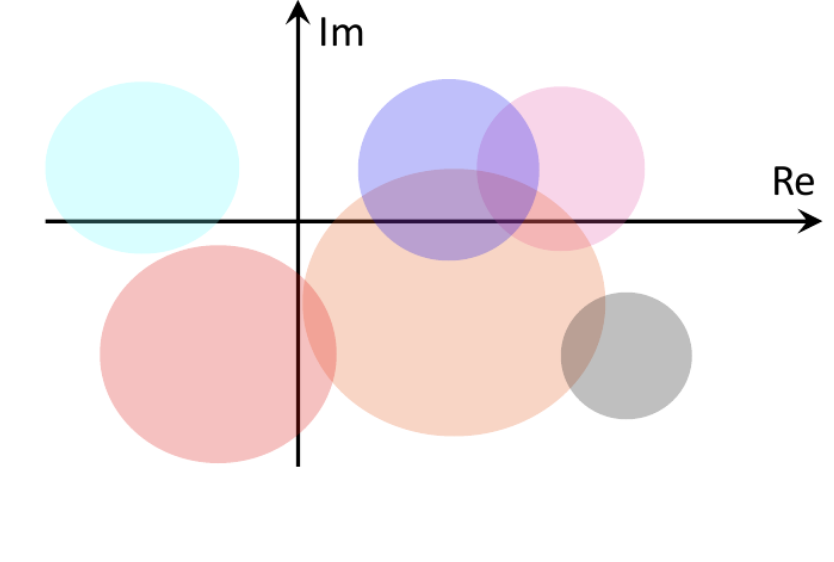
\includegraphics[width=.9\linewidth]{./img/gershgoren-diagonally-dominant.png}
\end{center}


\section{הגדרות בסיסיות ותכונות}
\label{sec:org4eec922}
\subsection{מטריצה חיובית מוגדרת (PD)}
\label{sec:org3315b92}
מטריצה \(K\) כך שמתקיים:
\[
\forall \underline{x} \ne 0,\ \ \underline{x}^TK\underline{x} > 0
\]
מטריצה כזו היא בהכרח לא סינגורית (היא הפיכה).

\subsection{מטריצה חיובית חצי מוגדרת (PSD)}
\label{sec:org70eab09}
מטריצה \(K\) כך שמתקיים:
\[
\forall x \ne 0,\ \ \underline{x}^TK\underline{x} \ge 0
\]

\subsection{מטריצת Gram}
\label{sec:org23607c9}
מטריצה \(K\) היא גראם אם קיימת \(A\) כך ש-\(K = A^TA\).

מטריצת גראם היא בהכרח חיובית חצי-מוגדרת.

\begin{itemize}
\item אם עמודות \(A\) בת״ל אז \(K\) היא גם חיובית מוגדרת.

\item אם \(C\) חיובית מוגדרת  ועמודות \(A\) בת״ל אז \(A^TCA\) היא חיובית מוגדרת.
\end{itemize}

\subsection{מטריצת Pseudo Inverse}
\label{sec:orgcdc3f6b}
עבור מטריצה \(A\) בעלת דרגה מלאה, מגדירים: \$A\textsuperscript{\textdagger{}} = \left( A\textsuperscript{TA} \right)\textsuperscript{-1}A\textsuperscript{T}

ובהקשר של פירוק SVD: \(A^{\dagger} = V \left( \Sigma^T\Sigma \right)^{-1} \Sigma^T U^T = V \Sigma^{\dagger}U^T\)

\subsection{היפוך מוכלל של מטריצה אלכסונית}
\label{sec:org583cdb9}

\(\begin{bmatrix}
\sigma_{1}  & 0 & 0 & 0 \\
0           & \sigma_{2} & 0 & 0 \\
0           & 0 & \sigma_{3} & 0 \\
0           & 0 & 0 & 0 \\
0           & 0 & 0 & 0 \\
0           & 0 & 0 & 0
 \end{bmatrix}^{\dagger} \triangleq \begin{bmatrix}
\frac{1}{\sigma_{1}}  & 0 & 0 & 0 & 0 & 0 \\
0           & \frac{1}{\sigma_{2}} & 0 & 0 & 0 & 0 \\
0           & 0 & \frac{1}{\sigma_{3}} & 0 & 0 & 0 \\
0           & 0 & 0 & 0 & 0 & 0
 \end{bmatrix}\)

\subsection{מספר מצב של מטריצה ריבועית}
\label{sec:org4fae357}
מספר מצב של מטריצה \(A_{n \times n}\) מוגדר ע״י \(\kappa \left\{ A \right\} = \frac{\sigma_1}{\sigma_n}\).
מספר המצב מייצג את הנטייה של המטריצה להיות סינגולרית:
\begin{itemize}
\item אם \(\kappa \left\{ A \right\} = 1\), המטריצה אורתונורמלית עד כדי קבוע.
\item אם \(\kappa \left\{ A \right\}\) נוטה ל-\(\infty\), מדובר במטריצה סינגולרית.
\end{itemize}


\section{גזירת ביטויים מטריציים וקטוריים}
\label{sec:orga93b22d}
\begin{itemize}
\item \(\nabla \|A\underline{x}-\underline{b}\|_2^2 = 2A^T \left( A\underline{x}-\underline{b} \right)\)
\end{itemize}




\section{אלגברה א׳}
\label{sec:org455b9e8}
\subsection{מטריצות}
\label{sec:org1b4c8b4}
\subsubsection{משפט: הכפלה במטריצות הפיכות משמאל לא משנה את מרחב השורה}
\label{sec:org9a62b5b}
(המערכות שקולות)


\section{כמויות חישובים}
\label{sec:org122337c}
\begin{center}
\begin{tabular}{ll}
תהליך & כמות פעולות\\\empty
\hline
החלפה קדמית/אחורה & \(\frac{1}{2}n^{2}\)\\\empty
פירוק \(LU\) & \(\frac{n^{3}}{3}\)\\\empty
היפוך מטריצה & \(4 \frac{n^3}{3}\)\\\empty
פירוק צ׳ולסקי יעיל & \\\empty
תהליך Gram-Schmidt & \(nL^2\)\\\empty
\end{tabular}
\end{center}
\end{document}